\chapter{药物效应动力学}

药物效应动力学(pharmacodynamics)的基本内容:药理作用,作用机制,临床应用和不良反应。

\section{药物作用的基本规律}

\subsection{药物的作用与效应}

药理作用(action):药物与机体的初始作用,如肾上腺素与肾上腺素α、β受体的结合并激动受体。

药理效应(effect):指药物作用产生的效应,肾上腺素与肾上腺素α、β受体的结合并激动受体,导致心率加快、血管收缩、血压升高等作用。

方式:直接作用或间接作用;全身作用或局部作用。

(一)药物效应的基本类型

(1)兴奋(stimulation):使器官、组织或细胞的活动增强。

(2)抑制(inhibition):使机体器官、组织或细胞的活动减少。

(3)亢进(augmentation):使有关组织或细胞活动过度兴奋。

(4)麻痹(paralysis):使有关组织、器官或细胞过度抑制,失去反应。

(5)衰竭(failure):使有关组织、器官或细胞由兴奋过度转为抑制。

(二)药物作用的选择性

药物作用的选择性(selectivity):指药物在一定的剂量首先对某一组织或器官产生作用,而对其他组织或器官无作用。

选择性可以是药效学的原因,比如药物受体的分布不均;也可以是药动学的原因,如药物在不同组织器官中的浓度不同。

\subsection{药物的治疗作用与不良反应}

(一)治疗作用

治疗作用(therapeutic
effect):指药物所引起的与用药目的一致的作用,是有利于防病、治病的作用。

对因治疗(etiological treatment):用药目的在于消除原发致病因素。

对症治疗(symptomatic treatment):用药目的在于改善疾病症状。

补充疗法(supplement therapy):又称替代疗法(replacement
therapy),对体内营养或代谢物质不足给予补充。

(二)不良反应

药理学上的不良反应(adverse drug reaction,
ADR),是指使用药物后出现的与用药目的无关并给病人带来不适或危害的反应。这与WHO《医用产品安全性检验》、我国《药品不良反应检测管理办法》中的不良反应的定义(强调是在正常剂量下产生)略有不同。

1.副反应(side reaction)

药物在治疗剂量下出现的与治疗目的无关的作用。与药物作用的选择性不高有关,往往是不可避免的,而且可以随着治疗目的的改变而发生变化。

如阿托品抑制腺体分泌,用于麻醉抑制呼吸道腺体分泌时,它加快心率的作用就成为引起心动过速等副作用;如果用于心动过缓,它抑制腺体分泌的作用就成为引起口干的副作用(图\ref{fig2-1})。

\begin{figure}[!htbp]
 \centering
 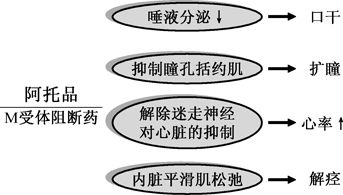
\includegraphics{./images/Image00004.jpg}
 \captionsetup{justification=centering}
 \caption{阿托品的作用}
 \label{fig2-1}
  \end{figure} 

2.毒性反应或毒性作用(toxic reaction, toxicity)

指用量过大或用药时间过长,对机体功能、形态产生的损害作用。毒性反应往往是药物作用的延伸,是可以预料和避免的。

毒性反应可分为急性毒性(acute toxicity)和慢性毒性(chronic
toxicity)。急性毒性指短时间内大剂量用药对机体产生损害。慢性毒性指长期使用药物后对机体产生损害。

有些药物会引起一些特殊毒性:①致畸作用(teratogenesis),如转换酶抑制剂、阿司匹林等药物可致畸胎;②致癌作用(carcinogenesis),如己烯雌酚、乙双吗啉;③致突变作用(mutagenesis)。

3.后遗效应(residual effect)

停药后残留药物引起的生物效应。

如巴比妥类和苯二氮䓬类催眠药往往会引起次晨头晕、困倦。长期用糖皮质激素可能导致肾上腺皮质功能低下,停药后可持续数月。

4.停药反应(withdrawal reaction)

也称回跃反应(rebound
reaction),指突然停药后原有疾病加重。如:长期服用可乐定停药次日血压即急剧升高。

5.继发反应(secondary reaction)

是指继发于药物治疗作用之后的不良反应。

常见的有:二重感染(supra-infection)、治疗房颤后的栓塞等。

6.变态反应(allergic reaction)

也称过敏反应(hypersensitive
reaction),是指药物对少数过敏体质病的人引起的病理性免疫反应,与药物的剂量和药理作用无关,有时很小量即可引起严重的变态反应。

药物、药物代谢产物或药物中的杂质是半抗原与机体的蛋白质结合后形成全抗原,刺激机体发生免疫反应。

7.特异质反应(idiosyncrasy)

指有特殊遗传缺陷的病人对某种药物反应异常增高所导致的不良反应。如遗传性G-6-PD(葡萄糖-6磷-酸脱氢酶)缺乏者服用磺胺类药物后可发生溶血性贫血。

8.药物依赖性(drug dependence)

指用药后所产生的一种强迫要求连续或定期使用该药的行为或其他反应,分为生理依赖性和精神依赖性两类。

(1)生理依赖性(physical
dependence),是指连续应用药品后,机体所发生的一种适应状态,此时机体需有足量药品的支持,方能处于正常功能状态。一旦停药,机体的生理功能就会紊乱,出现戒断症状(abstinence
syndrone)。吗啡、哌替啶、地西泮等药品停用时会引起程度不同的戒断症状。

(2)精神依赖性(psychic
dependence),也称成瘾(addiction):反复应用麻醉药品或精神药品后所产生的欣快、舒适、满足、安乐、幻觉、激动、刺激等感受,促使应用者产生渴求连续用药的欲望和不择手段的“觅药行为”。中断用药后,仅感主观心理上不适而并不引起戒断症状,常见的如可卡因、印度大麻等。

药物依赖性危害较大,已成为严重的社会问题。我国政府已颁布《麻醉药品管理办法》和《精神药品管理办法》,需按这两个管理办法对此类药品严加管理、严格控制、严禁滥用,以达合理使用的目的。

\subsection{量-效关系}

量-效关系(dose-effect
relationship),指药理效应的强弱与其剂量大小或浓度高低呈一定关系。药理效应按性质分为量反应和质反应。

1.量反应与量反应曲线

量反应(graded
response):效应的强弱呈连续增减的变化,可用具体数量或最大反应的百分率表示。可以在单一生物体上观察药物的作用,作用强度通常用数量单位表示。

量-效曲线(dose-effect
curve):以药理效应的强度为纵坐标,药物剂量或浓度为横坐标作图表。

\begin{figure}[!htbp]
 \centering
 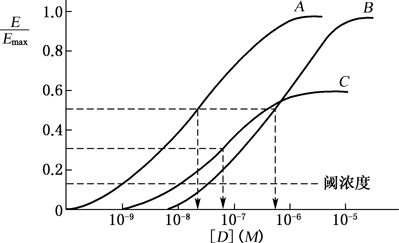
\includegraphics{./images/Image00005.jpg}
 \captionsetup{justification=centering}
 \caption{量-效关系的曲线}
 \label{fig2-2}
  \end{figure} 

阈剂量(浓度):即最小有效量(浓度)。

最大效应(maximum
efficacy):也称效能,即药物所能产生的最大效应,反映内在活性。

效应强度(potency):也称强度,指药物产生等效作用(通常为产生50%的效应)所需的剂量或浓度。反映药物与受体的亲合力;效价高的药物所需剂量较小。

2.质反应及其量效曲线

质反应:指在一群体中,药物引起某一效应以阳性(或阴性)反应出现的频数或百分率表示。

\begin{figure}[!htbp]
 \centering
 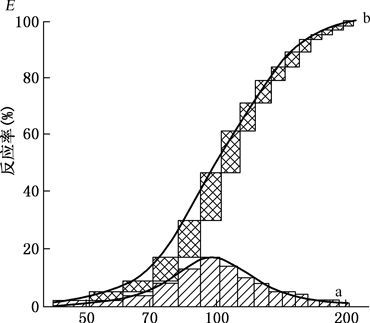
\includegraphics{./images/Image00006.jpg}
 \captionsetup{justification=centering}
 \caption{质反应与质反应曲线}
 \label{fig2-3}
  \end{figure} 

半数有效量(50% effective dose,
ED50):使群体中半数个体出现某一效应的药物剂量。

半数致死量(50% lethal dose, LD50):使实验动物死亡一半的药物剂量。

\begin{figure}[!htbp]
 \centering
 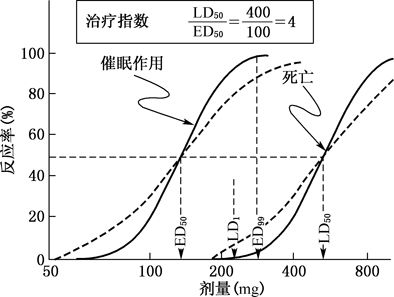
\includegraphics{./images/Image00007.jpg}
 \captionsetup{justification=centering}
 \caption{治疗指数}
 \label{fig2-4}
  \end{figure} 

药物安全性评价指标:

(1)治疗指数(therapeutic index, TI):TI=LD\textsubscript{50}
/ED\textsubscript{50} 。

(2)安全范围(margin of safety):LD\textsubscript{5}
/ED\textsubscript{95} 。

(3)可靠安全系数:LD\textsubscript{1} /ED\textsubscript{99} 。

\subsection{构效关系}

药理作用的特异性取决于药物的化学结构,即构效关系(structure activity
relationship, SAR)。构效关系是计算机辅助设计药物的主要依据。

\section{药物作用机制}

药物作用的靶点可以是:①受体;②酶;③离子通道;④转运体;⑤免疫系统;⑥基因和转录因子。

\section{受  体}

\subsection{受体与配体}

受体(receptor):是一类能介导细胞信号传导,识别环境中某种特定微量化学物质并与之选择性结合,通过信息放大系统,引起生物效应的功能蛋白质。

配体(ligand):能与受体特异性结合的物质。配体可分为内源性配体(如激素、神经递质或细胞因子)和外源性配体(如药物)。受体均有相应的内源性配体。

药物和受体的结合方式:①离子键;②氢键;③范德华引力;④共价键。除了共价键结合得比较牢固为不可逆结合外,其他三种结合力不牢固,都是可逆的结合。

药物与受体结合的特点:

(1)特异性 不同分子结构的药物与不同的受体结合,具有选择性。

(2)灵敏性 也叫亲和性。极低浓度(1pmol~1nmol/L)的药物就可以与受体结合并引起效应。

(3)饱和性与竞争性 受体的数量是有限的,通常膜受体的浓度为10fmol/mg。高浓度的药物可以充分结合受体,使效应达到饱和。与同一受体结合的药物同时存在时,可以发生竞争。

(4)多样性 即同一种受体可以有很多亚型。

\subsection{受体与药物相互作用的学说}

受体与药物相互作用的学说有:

1.占领学说(occupation theory)

占领学说的主要内容为:

(1)受体(R)与配体(L)之间的相互作用是可逆的。

(2)生物效应与被占领受体的量成正比,结合与效应间呈线性关系,当全部受体被占领时就会产生最大效应。

(3)与受体结合的配体只占总配体的极小部分([配体]≫[受体]),因此当反应达到平衡时,游离配体浓度接近总体基浓度。

2.速率学说(rate theory)

药物的效应与受体的解离速率有关,激动剂的解离速度快。

3.二态模型理论(two model theory)

受体有两种存在方式------激活型和失活型。

4.储备受体学说(reserve receptor theory)

受体中有一部分储备受体(spare receptor, silent
receptor),通常处于空闲状态。

其中占领学说是主要的,其他学说是对占领学说的修正。

Ariens于1954年对占领学说作了重要的补充和修正,即药物与受体结合后产生效应的能力------亲合力和内在活性。药物------受体相互作用并引发效应是由两步组成的:

(1)亲合力(affinity):与受体结合的能力。

(2)内在活性(intrinsic
activity):药物产生最大效应的能力,以α表示。当α=1,药物为激动剂(agonist);当0<α<1,药物为部分激动剂(partial
agonist, PA);当α=0,药物为拮抗剂(antagonist)。

\subsection{激动药}

激动药(agonist):既有亲合力又有完全内在活性的药物,它们能与受体结合并激动受体而产生效应(α=1)。

\begin{figure}[!htbp]
 \centering
 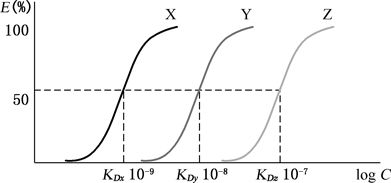
\includegraphics{./images/Image00008.jpg}
 \captionsetup{justification=centering}
 \caption{激动剂}
 \label{fig2-5}
  \end{figure} 

X、Y、Z三药的内在活性(E\textsubscript{max}
)相等,但与受体的亲合力不等,X>Y>Z

拮抗药(antagonist):有较强的亲合力能与受体结合,但无内在活性(α=0),不能激动受体的药物,可抑制激动剂与受体结合的药物。

根据拮抗药与受体结合是否有可逆性而将其分为竞争性拮抗药(competitive
antagonists)和非竞争性拮抗药(noncompetitive antagonists)

1.竞争性拮抗药(competitive antagonists)

可逆性与激动药竞争和相同的受体结合,其特点是量效曲线右移和最大效应不变。

\begin{figure}[!htbp]
 \centering
 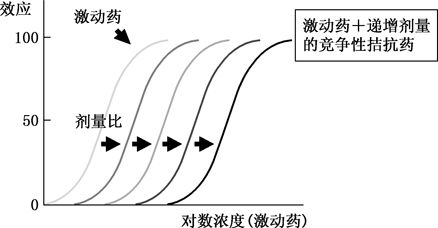
\includegraphics{./images/Image00009.jpg}
 \captionsetup{justification=centering}
 \caption{激动剂与竞争性拮抗剂}
 \label{fig2-6}
  \end{figure} 

拮抗参数(antagonist parameter,
pA2):使激动药浓度增加一倍时引起原有激动药反应时的拮抗药摩尔浓度的负对数。

剂量比(dose ratio)为2时,即$\frac{\text{加了拮抗剂后激动剂浓度}[C^\prime]}{\text{无拮抗剂时激动剂浓度}[C]}=2$
时

竞争性拮抗药浓度的负对数,pA2=-log{[}A{]}。

2.非竞争性拮抗药(non-competitive antagonists)

与受体结合非常牢固或与受体结合后能改变效应器官的反应性,使激动药量效曲线右移和最大效应降低。

减活指数(pA2′):使激动药浓度增加一倍时引起原有激动药反应时的非拮抗药摩尔浓度的负对数。

\begin{figure}[!htbp]
 \centering
 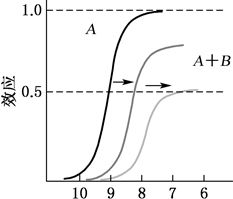
\includegraphics{./images/Image00011.jpg}
 \captionsetup{justification=centering}
 \caption{非竞争性拮抗}
 \label{fig2-7}
  \end{figure} 

\begin{figure}[!htbp]
 \centering
 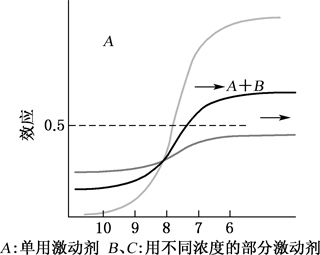
\includegraphics{./images/Image00012.jpg}
 \captionsetup{justification=centering}
 \caption{部分激动剂}
 \label{fig2-8}
  \end{figure} 

(1)部分激动药(partial
agonist)有较强的亲合力,但内在活性不强(0<α<1),即表现部分阻断作用。

(2)部分激动药------在激动药浓度较低时与激动药产生协同作用;在激动药浓度较高时则产生拮抗作用。

(3)反向激动药(inverse
agonist)具有与激动剂相反的内在活性。现在认为G蛋白偶联受体通常处于一种自发的激动状态。这种自发激动状态可以被反向激动剂抑制。

\begin{figure}[!htbp]
 \centering
 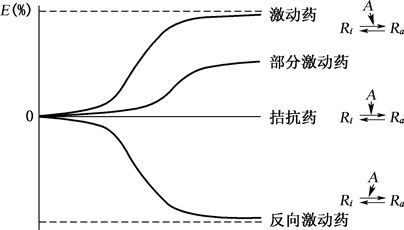
\includegraphics{./images/Image00013.jpg}
 \captionsetup{justification=centering}
 \caption{反向激动剂}
 \label{fig2-9}
  \end{figure} 

\subsection{受体与药物反应动力学基本公式}

$$D+R\xrightarrow{K}DR\rightarrow\rightarrow\cdots\rightarrow E$$
$$\frac{E}{E_{\text{max}}}=\frac{[DR]}{[Rt]}=\frac{[D]}{K_d+[D]}$$

当[D]≫K\textsubscript{d} ,$\frac{[DR]}{[Rt]}=100\%$
,E=E\textsubscript{max}

当$\frac{[DR]}{[Rt]}=50\%$
时,$\frac{[D]}{K_d+[D]}=50\%=\frac{1}{2}$

K\textsubscript{d} +D=2D

K\textsubscript{d} =D

K\textsubscript{d} 为解离常数,K\textsubscript{d}
值是占领受体总数时一半(或引起50%最大效应时)所需药物的摩尔浓度[D]。K\textsubscript{d}
越小,说明药物占领受体总数一半时或引起50%最大效应时所需的药物浓度低,药物与受体的亲合力大,亲合力=1/K\textsubscript{D}
。

亲合力指数(pD\textsubscript{2}
):即解离常数的负对数,pD\textsubscript{2} =-logK\textsubscript{D}
。pD\textsubscript{2} 值越大,药物的亲合力越大。

\subsection{受体的调节}

1.向下调节(down-regulation)

长期使用受体激动剂可以减少受体数量,这称为受体向下调节。受体向下调节可能是激动剂长期应用后产生耐受性的机制之一。耐受性还可能是受体的敏感性下降或信号传递系统阻滞。

2.向上调节(up-regulation)

长期使用受体拮抗剂可以增加受体数量,这称为受体向上调节。受体向上调节可能是拮抗剂长期应用后受体增敏、产生反跳现象或戒断综合征的机制之一。受体增敏还可能是受体的敏感性增加或信号传递系统增强所致。

\subsection{受体的分类及细胞内信号传导途径}

1.G蛋白耦联受体(G protein coupled receptor)

肾上腺素α、β受体,胆碱能M受体,组胺H\textsubscript{1}
受体等都属于这类受体。

\begin{figure}[!htbp]
 \centering
 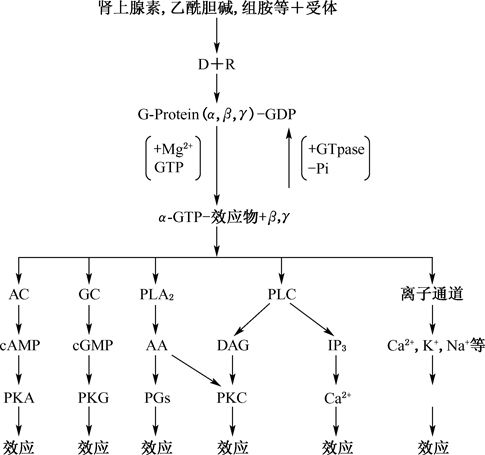
\includegraphics{./images/Image00019.jpg}
 \captionsetup{justification=centering}
 \caption{G蛋白耦联受体的信号传递}
 \label{fig2-10}
  \end{figure} 

2.配体门控离子通道受体(ligand-gated ion channel receptor)

胆碱能N\textsubscript{N} 受体、γ-氨基丁酸受体属于配体门控离子通道受体。

\begin{figure}[!htbp]
 \centering
 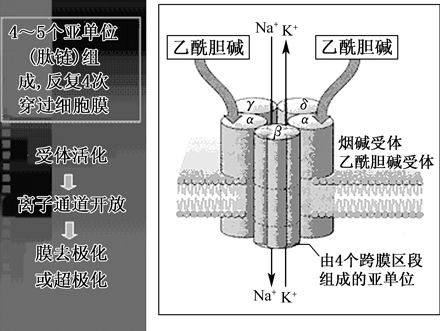
\includegraphics{./images/Image00020.jpg}
 \captionsetup{justification=centering}
 \caption{配体门控离子通道受体}
 \label{fig2-11}
  \end{figure} 

3.酶活性受体

如:酪氨酸激酶受体(tyrosine kinase receptors, receptors with tyrosine
kinase
activity),胰岛素、胰岛素样生长因子。很多生长因子和一些淋巴因子都是通过这类受体传递信号。

\begin{figure}[!htbp]
 \centering
 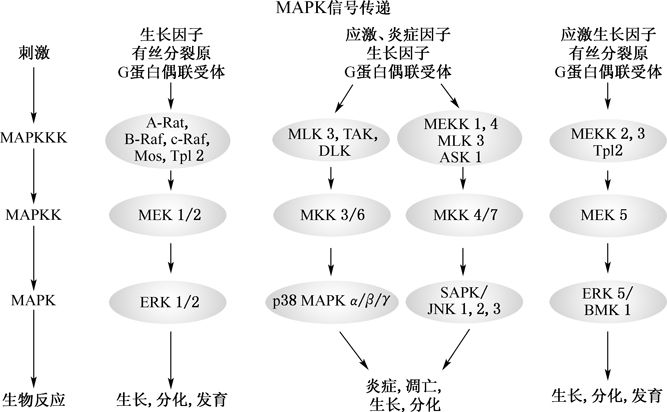
\includegraphics{./images/Image00021.jpg}
 \captionsetup{justification=centering}
 \caption{MAPK的信号传递}
 \label{fig2-12}
  \end{figure} 

4.细胞内受体(intracellular receptor)

这类受体存在于细胞内或细胞核中(转录因子家族的一部分),有配体识别结合区和DNA结合区。产生效应较慢(数小时)。

糖皮质激素、盐皮质激素、雄激素、孕激素、雌激素、甲状腺素(T\textsubscript{3}
及T\textsubscript{4} )和Vit D等,除甲状腺素外均为类固醇化合物。

\begin{figure}[!htbp]
 \centering
 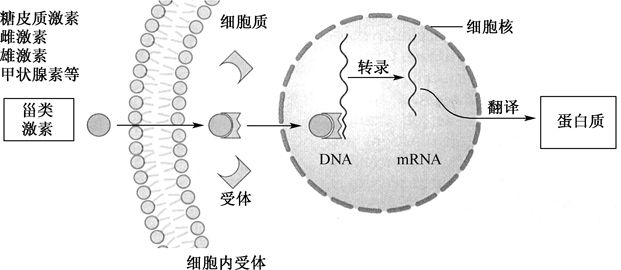
\includegraphics{./images/Image00022.jpg}
 \captionsetup{justification=centering}
 \caption{细胞内受体的信号传递}
 \label{fig2-13}
  \end{figure} 

\section*{大纲要求}

1.掌握药物剂量和效应关系。

2.掌握药物不良反应的种类及临床表现。

3.掌握作用于受体的药物分类。

